%%%%%%%%%%%%%%%%%%%%%%%%%%%%%%%%%%%%%%%%%
% Jacobs Landscape Poster
% LaTeX Template
% Version 1.0 (29/03/13)
%
% Created by:
% Computational Physics and Biophysics Group, Jacobs University
% https://teamwork.jacobs-university.de:8443/confluence/display/CoPandBiG/LaTeX+Poster
%
% Further modified by:
% Nathaniel Johnston (nathaniel@njohnston.ca)
%
% This template has been downloaded from:
% http://www.LaTeXTemplates.com
%
% License:
% CC BY-NC-SA 3.0 (http://creativecommons.org/licenses/by-nc-sa/3.0/)
%
%%%%%%%%%%%%%%%%%%%%%%%%%%%%%%%%%%%%%%%%%

%----------------------------------------------------------------------------------------
%	PACKAGES AND OTHER DOCUMENT CONFIGURATIONS
%----------------------------------------------------------------------------------------

\documentclass[final]{beamer}

% \usepackage[scale=1.24]{beamerposter} % Use the beamerposter package for laying out the poster
\usepackage[scale=0.8]{beamerposter}

\usetheme{confposter} % Use the confposter theme supplied with this template

\setbeamercolor{block title}{fg=ngreen,bg=white} % Colors of the block titles
\setbeamercolor{block body}{fg=black,bg=white} % Colors of the body of blocks
\setbeamercolor{block alerted title}{fg=white,bg=dblue!70} % Colors of the highlighted block titles
\setbeamercolor{block alerted body}{fg=black,bg=dblue!10} % Colors of the body of highlighted blocks
% Many more colors are available for use in beamerthemeconfposter.sty

%-----------------------------------------------------------
% Define the column widths and overall poster size
% To set effective sepwid, onecolwid and twocolwid values, first choose how many columns you want and how much separation you want between columns
% In this template, the separation width chosen is 0.024 of the paper width and a 4-column layout
% onecolwid should therefore be (1-(# of columns+1)*sepwid)/# of columns e.g. (1-(4+1)*0.024)/4 = 0.22
% Set twocolwid to be (2*onecolwid)+sepwid = 0.464
% Set threecolwid to be (3*onecolwid)+2*sepwid = 0.708

\newlength{\sepwid}
\newlength{\onecolwid}
\newlength{\twocolwid}
\newlength{\threecolwid}
% \setlength{\paperwidth}{48in} % A0 width: 46.8in
% \setlength{\paperheight}{36in} % A0 height: 33.1in
\setlength{\paperwidth}{36in} % A0 width: 46.8in
\setlength{\paperheight}{24in} % A0 height: 33.1in
\setlength{\sepwid}{0.024\paperwidth} % Separation width (white space) between columns
% \setlength{\onecolwid}{0.22\paperwidth} % Width of one column
% \setlength{\twocolwid}{0.464\paperwidth} % Width of two columns
% \setlength{\threecolwid}{0.708\paperwidth} % Width of three columns
\setlength{\onecolwid}{0.3013\paperwidth} % Width of one column
\setlength{\twocolwid}{0.6026\paperwidth} % Width of two columns
\setlength{\threecolwid}{0.904\paperwidth} % Width of three columns
\setlength{\topmargin}{-0.5in} % Reduce the top margin size
%-----------------------------------------------------------

\usepackage{graphicx}  % Required for including images
\usepackage{booktabs} % Top and bottom rules for tables
\usepackage{amssymb}
\usepackage{amsthm}
\usepackage{amsmath}
\usepackage{mathrsfs}
\usepackage{algorithm}
\usepackage{algorithmic}
\usepackage{grffile}

\newcommand{\bx}{\mathbf{x}}
\newcommand{\R}{\mathbb{R}}
\newcommand{\E}{\mathbb{E}}
\newcommand{\D}{\mathscr{D}}
\newcommand{\N}{\mathscr{N}}
\newcommand{\by}{\mathbf{y}}
\newcommand{\var}{\mathrm{var}}
\newcommand{\cov}{\mathrm{cov}}
\DeclareMathOperator*{\argmin}{\arg\!\min}

\newtheorem{conjecture}{Conjecture}
% \newtheorem{theorem}{Theorem}
\newtheorem{experiment}{Experiment}

% inline theorem
\makeatletter
\setbeamertemplate{theorem begin}
  {\usebeamercolor[fg]{thcolor}% for the heading
  {\bfseries\inserttheoremname~}%
  \ifx\inserttheoremaddition\@empty\else(\inserttheoremaddition)\ \fi%
  \hspace{.01em}\normalfont\usebeamercolor[fg]{thcolor}% for the body
  }
\setbeamertemplate{theorem end}{}
\makeatother
%----------------------------------------------------------------------------------------
%	TITLE SECTION
%----------------------------------------------------------------------------------------

\title{Novel Sampling Using Stochastic Gradient Descent} % Poster title

\author{Yu Wang and Weixin Cai} % Author(s)

\institute{Department of Statistics, UC Berkeley} % Institution(s)

%----------------------------------------------------------------------------------------

\begin{document}



\addtobeamertemplate{block end}{}{\vspace*{2ex}} % White space under blocks
\addtobeamertemplate{block alerted end}{}{\vspace*{2ex}} % White space under highlighted (alert) blocks

\setlength{\belowcaptionskip}{2ex} % White space under figures
\setlength\belowdisplayshortskip{2ex} % White space under equations

\begin{frame}[t] % The whole poster is enclosed in one beamer frame

\begin{columns}[t] % The whole poster consists of three major columns, the second of which is split into two columns twice - the [t] option aligns each column's content to the top

\begin{column}{\sepwid}\end{column} % Empty spacer column

\begin{column}{\onecolwid} % The first column

%----------------------------------------------------------------------------------------
%	OBJECTIVES
%----------------------------------------------------------------------------------------

\begin{alertblock}{Main results}

% \centerline{ \bf{ Aim of study}}

\begin{enumerate}
\item Stochastic gradient descent (SGD) as a class of efficient Markov chain sampler
\item Derived the stationary distribution
\item Fast sampler for any Bayesian posteriors
\item Derived upper bound on the mixing time based on convergence results
\end{enumerate}

\end{alertblock}

%----------------------------------------------------------------------------------------
%   MOTIVATION
%----------------------------------------------------------------------------------------

\begin{block}{Motivation}

\begin{itemize}
\item Sampling from posterior distribution is crucial in various statistical techniques
\item Posterior can be hard to sample  (hurdle a lot of applications)
\item SGD can be viewed as a Markov chain
\item Property as a Markov chain seems to be largely overlooked
\item Stationary distribution? Mixing time? Mixing time relationship with convergence rate?
\end{itemize}

\end{block}

%------------------------------------------------
%
%----------------------------------------------------------------------------------------
%	INTRODUCTION
%----------------------------------------------------------------------------------------

\begin{block}{SGD Sampling Algorithm}
Suppose we would like to sample from a distribution $p(\bx)\in \D(\R^p) \propto f(\bx)$. 
\begin{algorithm}[H]
{\small
Given $f(x)$, 
\begin{algorithmic}\caption{Stochastic gradient descent (oracle)}\label{Alg:SGD}
\STATE {\bf Initialize} $ \bx^0$ arbitrarily;
\WHILE{burn-in period}
\STATE draw $a^t$ from Gaussian distribution $\N(\nabla \log f(\bx^k), \Sigma^{t})$.
\STATE
$\bx^{k+1} \gets \bx^k + (2\Sigma^t)^{-1} a^t$;
\STATE $k\gets k+1$;
\ENDWHILE
\STATE return $\bx^k$.
\end{algorithmic}}
\end{algorithm}


\end{block}

%----------------------------------------------------------------------------------------
%   REFERENCES
%----------------------------------------------------------------------------------------

\begin{block}{References}

\nocite{*} % Insert publications even if they are not cited in the poster
\small{\bibliographystyle{unsrt}
\bibliography{sample}\vspace{0.75in}}

\end{block}

%----------------------------------------------------------------------------------------

\end{column} % End of the first column

\begin{column}{\sepwid}\end{column} % Empty spacer column

\begin{column}{\onecolwid} % Begin a column which is two columns wide (column 2)

%------------------------------------------------

\begin{figure}
    \centering
    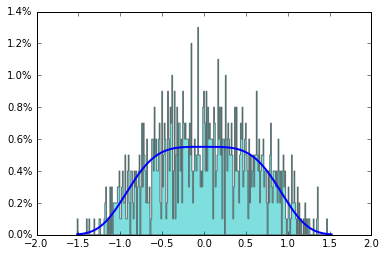
\includegraphics[width=.3\onecolwid]{../figure/case1_step_0.005_iter_1e3.png}
    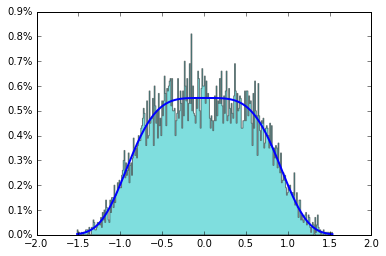
\includegraphics[width=.3\onecolwid]{../figure/case1_step_0.005_iter_1e4.png}
    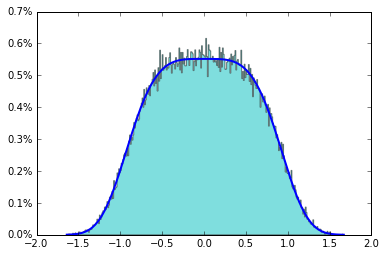
\includegraphics[width=.3\onecolwid]{../figure/case1_step_0.005_iter_1e5.png}\\
    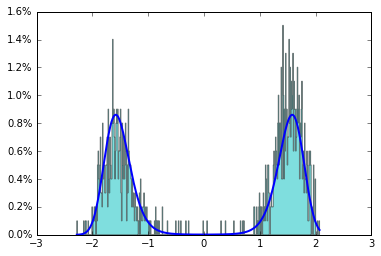
\includegraphics[width=.3\onecolwid]{../figure/case2_step_0.005_iter_1e3.png}
    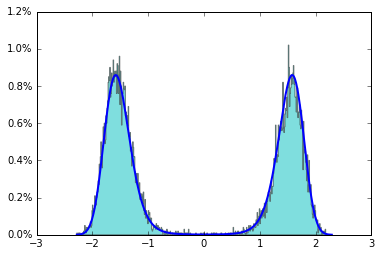
\includegraphics[width=.3\onecolwid]{../figure/case2_step_0.005_iter_1e4.png}
    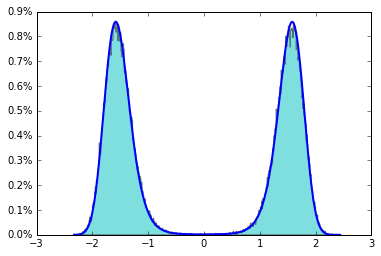
\includegraphics[width=.3\onecolwid]{../figure/case2_step_0.005_iter_1e5.png}\\
    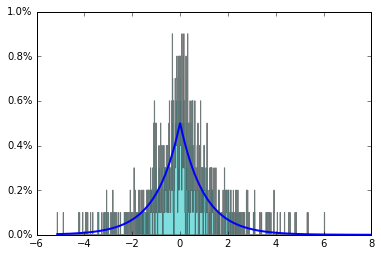
\includegraphics[width=.3\onecolwid]{../figure/case3_step_0.005_iter_1e3.png}
    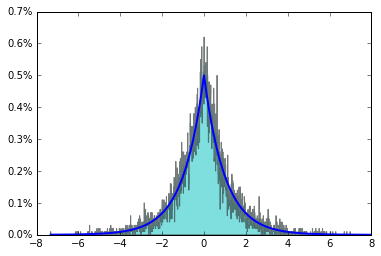
\includegraphics[width=.3\onecolwid]{../figure/case3_step_0.005_iter_1e4.png}
    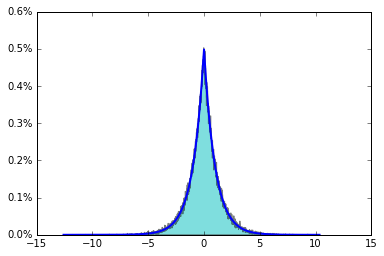
\includegraphics[width=.3\onecolwid]{../figure/case3_step_0.005_iter_1e5.png}
    \caption{Empirical stationary distribution using SGD. Different columns correspond to different samples sizes ($1e3$, $1e4$, and $1e5$). Different rows correspond to different distributions ($f_1(x) = \exp(-x^4)$, $f_2(x) = \exp(-(x^2 - 4)(x^2 - 1))$, $f_3(x) = \exp(-|x|)$.}
    \label{Fig:exp1}
\end{figure}

%----------------------------------------------------------------------------------------
%	MATERIALS
%----------------------------------------------------------------------------------------
\begin{block}{Stationary Distribution}
Will Algorithm 1 converge to the desired stationary distribution? Denote $p(\bx^{t+1}|\bx^t)$ to be the density function to obtain $\bx^{t+1}$ from $\bx^{t}$. 
The detailed balance condition holds approximately when $\|(\Sigma^t)^{-1}\|$ is small, i.e.,
\[
f(\bx^{t})p(\bx^{t+1}|\bx^t) = f(\bx^{t+1})p(\bx^{t}|\bx^{t+1}) ( 1 + O(\|(\Sigma^t)^{-1}\|^2)).
\]
That implies $f(\cdot)$ is indeed the stationary distribution of Algorithm 1. Simulation results can be found in Figure 1.
\end{block}


%----------------------------------------------------------------------------------------
%   ADDITIONAL INFORMATION
%----------------------------------------------------------------------------------------

\begin{block}{SGD As Posterior Sampler}
When $p(\theta)$ is the posterior distribution of some parameters given a set of data $X_1,\ldots, X_n$, i.e.,
\[
p(\theta) = \prod_{i=1}^n P(X_i|\theta) P(\theta),
\]
The noisy gradient step in Algorithm 1 can be estimated by subsampling:
\begin{theorem}[Central limit theorem]
Let $K$ be the subsampling size and $\eta_1,\ldots, \eta_K$ be samples drawing from $1,\ldots, n$ with replacement, then
\[
K^{-1}\sum_{i=1}^K (\nabla \log P(X_{\eta_i}|\theta^t) - \log P(\theta^t)) \sim \N(n^{-1} \nabla \log p(\theta) , K^{-1}\cov \nabla \log p(\theta)).
\]
\end{theorem}

See Figure 2 for the simulation result.

\end{block}

%----------------------------------------------------------------------------------------

\end{column} % End of the second column

\begin{column}{\sepwid}\end{column} % Empty spacer column

\begin{column}{\onecolwid} % The third column


%------------------------------------------------

\begin{figure}
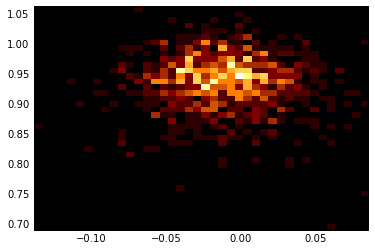
\includegraphics[width=0.5\linewidth]{../figure/simulation2_empirical.png}
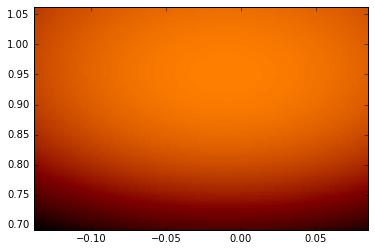
\includegraphics[width=0.5\linewidth]{../figure/simulation2_real.png}
\caption{Figure caption}
\end{figure}


%----------------------------------------------------------------------------------------
%   ADDITIONAL INFORMATION
%----------------------------------------------------------------------------------------

\begin{block}{Upper Bound On Mixing Time}
Mixing time correspon

\end{block}

%----------------------------------------------------------------------------------------
%	CONCLUSION
%----------------------------------------------------------------------------------------

\begin{block}{Conclusion}

\begin{itemize}
\item Proposed fast SGD sampler for posterior distributions. Computing the likelihood from the full data is intensive.
\item Proved accurate stationary distribution based on oracle results
\item Established connection between SGD and maximize \emph{a posteriori} (MAP)
\item Derived upper bound on mixing time
\item Future work: Finite sample rates of convergence for the mixing time
\end{itemize}

\end{block}

%----------------------------------------------------------------------------------------
%   ACKNOWLEDGEMENTS
%----------------------------------------------------------------------------------------

\begin{block}{Acknowledgements}

\small{\rmfamily{We would like to thank Professor Martin Wainwright for his inspiring teaching this semster. And we also greatly appreciate Arturo Fernandez and Jeffery Chan, our GSIs, for their devotion in this course.}} \\

\end{block}





%----------------------------------------------------------------------------------------
%	CONTACT INFORMATION
%----------------------------------------------------------------------------------------


\begin{block}{Contant Information}

\begin{itemize}
\item Email: \href{mailto:wang.yu@berkeley.edu, wcai@berkeley.edu}{\{wang.yu, wcai\}@berkeley.edu}
\end{itemize}


\end{block}

%----------------------------------------------------------------------------------------

\end{column} % End of the third column

\end{columns} % End of all the columns in the poster

\end{frame} % End of the enclosing frame

\end{document}
